\subsection{M.2.3 Variazione di costo}
\begin{figure}[H]
    \centering
    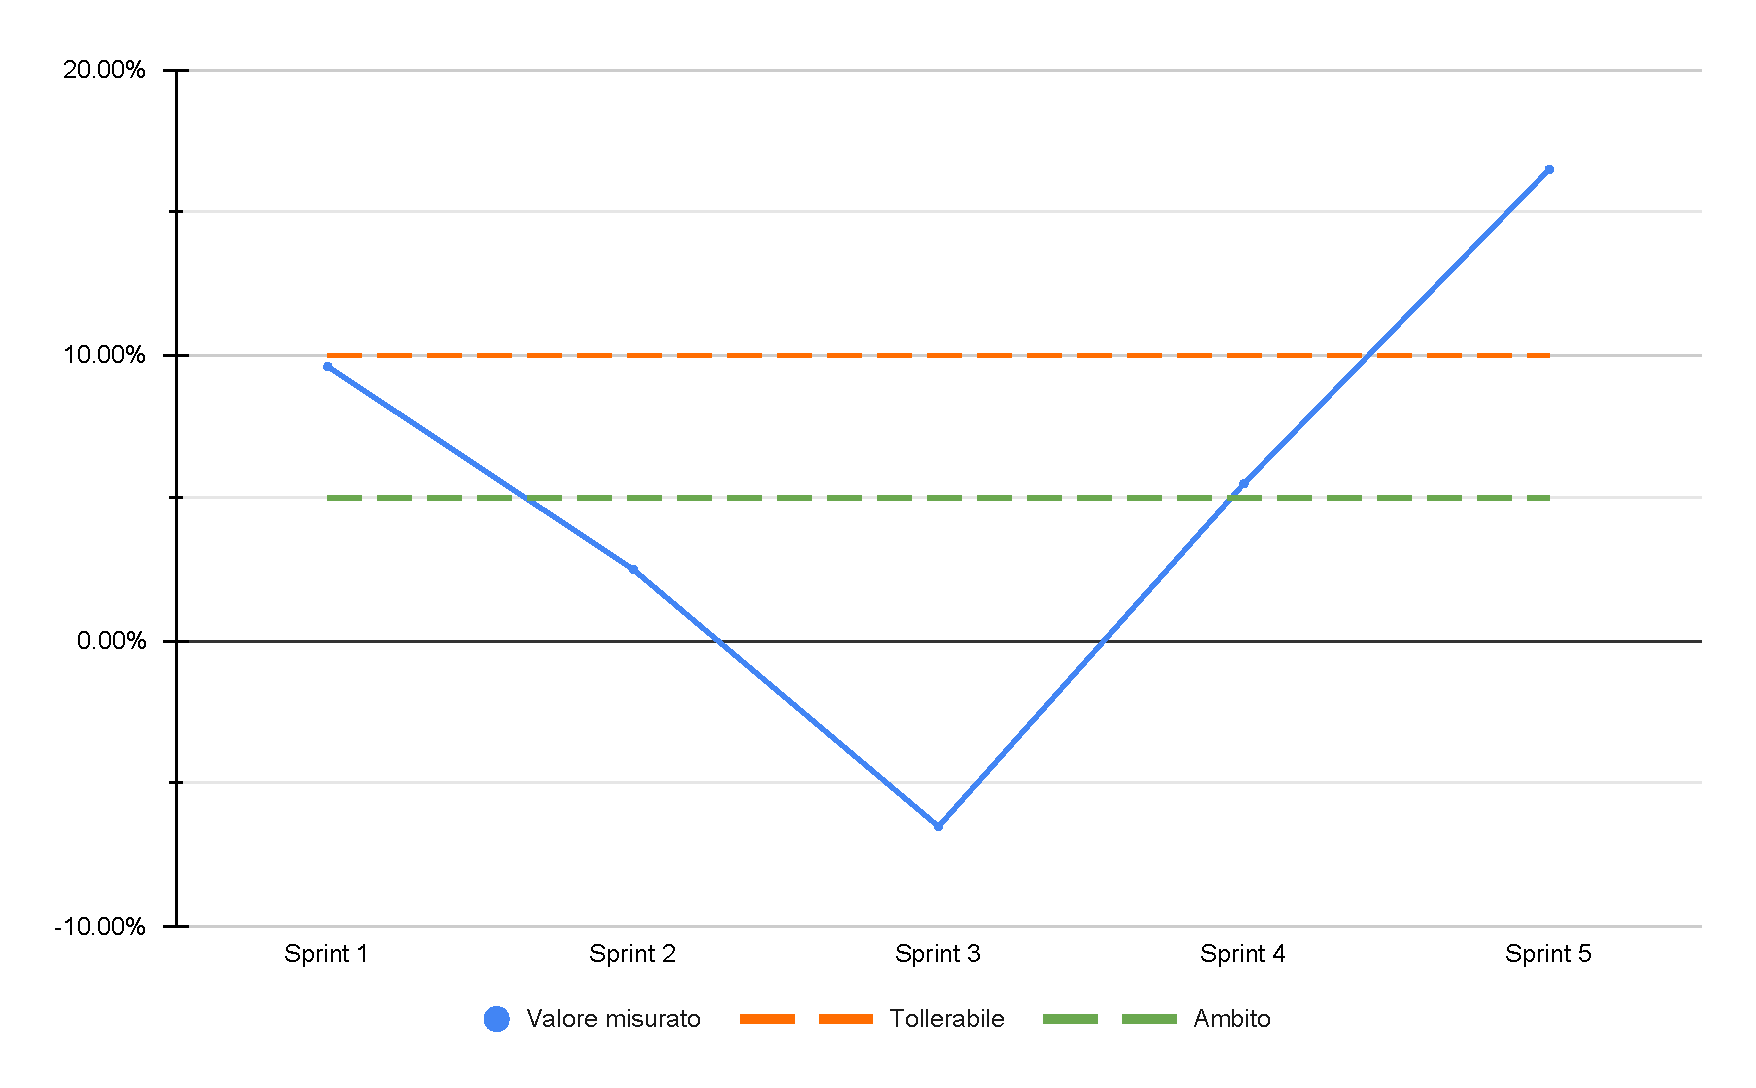
\includegraphics[width=0.8\textwidth]{assets/variazione_costo.pdf}
    \caption{M.2.3 Variazione di costo}
\end{figure}

\par Il grafico mostra come dal primo \glossario{sprint}, il gruppo abbia lavorato rispettando i costi proposti sul preventivo per lo \glossario{sprint}. Questo è visto sia in termini positivi che negativi, poiché una variazione di costo vicina alla soglia di tollerabilità, è anche indice di inesperienza sulla distribuzione dei ruoli e sulla gestione delle attività o di criticità che hanno rallentato i lavori, aumentando il costo complessivo dello \glossario{sprint}.
Durante gli \glossario{sprint} successivi, il gruppo ha lavorato in modo più efficiente, avvicinandosi sempre di più al costo preventivato. Dallo \glossario{sprint} 4, il grafico ha una nuova risalita dovuta ad un cambio di tecnologie che ha comportato un aumento dei costi al di sopra della soglia tollerabile. La tendenza generale del grafico, dal secondo \glossario{sprint} è comunque sempre rimasta compresa tra il valore ambito e il valore tollerabile. 